% March 26, 2013
% Latex templete for preparation of Project Report of Final Year of MCA Students
%
% In Latex any command starting with % treated as comment.

% ------------------------------------------------------------------------------------
% Packages (if any package not installed on ur PC, just connect internet and run ur file, packages automatically installed)
% Document type and packages required (required package information is in etcreport.sty 
\documentclass[12pt, oneside, a4paper]{report}
\usepackage{etcreport}
\usepackage{titlesec}
\titleformat{\chapter}[display]
{\normalfont\huge\bfseries}{\filright\chaptertitlename\ \thechapter}{20pt}{\Huge\centering}

%-----------------------------------------------------------------------------------
\begin{document}
% ---------------------------------------------------------------------------------
% Add following chpaters - create separate tex files - sample files are given- edit them or create ur own
% ---------------------------------------------------------------------------------
\thispagestyle{empty}
  %\thisfancyput(3.25in,-4.5in){%
   %\setlength{\unitlength}{1in}\fancyoval(7,9.5)}

   \begin{center}
   \Huge \bfseries \textcolor{black} {A}\\[.2cm]
   \Huge \bfseries \textcolor{black} {Project Report}\\[.2cm]
	\Huge \bfseries \textcolor{black} {on}\\[.2cm]
% Change in following Line - Name of Project Title
% ---------------------------------------------------------------------
   \huge \bfseries \textcolor{purple} {``Matricsv''}\\[.8cm]
   \Huge \bfseries \textcolor{black} {At}\\[.2cm]
   \Huge \bfseries \textcolor{black} {Sushilaai Web Solutions, Dhule}\\[.9cm]
% ---------------------------------------------------------------------
   \large \bfseries \textcolor{black} {Submitted By:}\\[.2cm]
% Change in following Line - Name of Project Developer% -----------------------------------------------------------------
     \Large \bfseries \textcolor{purple} {Hemanshu Sanjay Mahajan}\\[.8cm]
     \Large \bfseries \textcolor{black} {To}\\[.2cm]
      
\includegraphics[scale=0.5]{Title/111}\\[0.1cm]
      \Large \bfseries \textcolor{cyan} { Institute of Management Research and Development, Shirpur}\\[0.1cm]
  
      
% -----------------------------------------------------------------
   \Large \bfseries \textcolor{black} {KBC North Maharashtra University, Jalgaon }\\[.7cm]
   \large \bfseries \textcolor{black} {Guided By:}\\[.2cm]

% Change in following Line - Name of Project Guide
% ---------------------------------------------------------------------
   \Large \bfseries \textcolor{purple} {Prof. Sapana Yeshi.}\\[1cm]
% ---------------------------------------------------------------------
  
   \large \bfseries \textcolor{black} {  In the partial fulfillment of the requirement for the award of the degree of ‘ Integrated Master of Computer Application’}\\[0.12cm]
   
   \huge \bfseries \textcolor{purple} {2024-25}\\[0.1cm]
\end{center}
 % add titlepage (stored in Title folder)
\thispagestyle{empty}
%\thisfancyput(3.25in,-4.5in){%
%\setlength{\unitlength}{1in}\fancyoval(7,9.5)}
\begin{center}

\includegraphics[scale=0.5]{Certi/111}\\[0.1cm]
\normalsize \bfseries \textcolor{black} {R. C. Patel Educational Trust's}\\[0.1cm]
\LARGE \bfseries \textcolor{cyan} {R. C. Patel Institute of Management Research \& Development }\\[0.1cm]
\large \bfseries \textcolor{black} {Shirpur, Dist-Dhule 425405}\\[0.1cm]
----------------------------------------------------------------------------- \\[0.9cm]

\underline{\textit{\LARGE \textcolor{purple} {CERTIFICATE}}}\\[0.1cm]
\end{center}
\begin{flushleft}
\justifying
\begin{spacing}{2}
% Change in following Lines - Write ur Project Title, Names of Project Group Members  
% ---------------------------------------------------------------------------------


\textit{\large \textcolor{black}  This is to certify that Mr. Hemanshu Sanjay Mahajan, a final year student of \textbf {'Integrated Master of Computer Application'} from Institute of Management Research \& Development, Shirpur has successfully completed the project entitled \textbf{``Matricsv''} as a part of academic six month industrial training which is approved for degree of Master of Computer Application a post graduate course of \textbf {'KBC North Maharashtra University, Jalgaon'} during acadmic year 2024-25.}   \\[0.9cm]


 %---------------------------------------------------------------------------------
\end{spacing}
\noindent
%Date:\\[0.3cm]
%Place: Shirpur\\[1.6 cm] 
\textbf{Director \hspace{9cm} Examiner\\RCPET'S IMRD,\\ Shirpur}\\[1.5cm]
%\textbf{ Exa}\hspace{5.5cm} %\textbf{Examiner}

%-----certificate------

\newpage
\thispagestyle{empty}

\begin{center}
\vspace*{2cm}

\includegraphics[width=0.9\textwidth]{Certi/doraemon.png}
\end{center}



\end{flushleft}





% End of Certificate	% add Certificate (stored in Certi folder)
\thispagestyle{empty}
\begin{flushright}
\textit{\Large \textcolor{black} Acknowledgment}\
\rule{6in}{.1pt}\\[0.5cm]
\end{flushright}
\justifying
\begin{spacing}{1.5}
% Change following - write ur acknowledgement (sample is given u may use same.
% ---------------------------------------------------------------------------------
I take this opportunity to express my sincere thanks to \textbf{ Sushilaai web solutions, Dhule}  for providing me an opportunity to work in the organization. I also express my gratitude to \textbf{Mr.Digambar Shinde (Project Manager and Team Leader)} Sushilaai Web Solutions, Dhule who gave me the opportunity to work in Sushilaai Web Solutions. His prudent ideas of work, keen interest in developing the system and constant effort were a great source of inspiration for us me. He not only guided us on the technical aspect but his acknowledgement of marketing strategies helped us in broadening our perspective.\\
	 I express my thanks to \textbf { Mr.Digambar Shinde (Project Manager and Team Leader)}. for their valuable guidance and experienced suggestion, encouragement and support extended by them helped me in various stages where I needed help and suggestions.\\
	 I am thankful to \textbf{Dr. Vaishali Patil. (Director), Prof. M. N. Behere (Head Dept. of MCA), and Prof. Sapana Yeshi. (Project Guide),  } R. C. Patel Institute of Management Research and Development, Shirpur, for giving me his valuable guidance and encouragement during our course. I am thankful to the college staff for their constant encouragement.\\
	 Last but not least, I am thankful to all people who directly or indirectly contributed to make this project a success.\\
	%We would be failing in our duties if we do not make a mention of our family members including our parents for providing moral support, without which this work would not have been completed.%

	
 	
	
	
% Change in following Line - Name of Project Group members     
% -----------------------------------------------------------------
\begin{flushright}
\begin{spacing}{1}
\textbf{Thanks \& Regards}\\[.03cm]
\textbf{Hemanshu S. Mahajan}\\[.01cm]

\end{spacing}
\end{flushright}
\end{spacing}

 % add acknowledgement (stored in Ack folder)
%\thispagestyle{empty}
\begin{flushright}
\textit{\Large \textcolor{black} Abstract}\
\rule{6in}{.1pt}\\[0.5cm]
\end{flushright}
\justifying
\begin{spacing}{1.5}
Now a days, blind people can do more than anyone can Imagine. They can perform many computer applications, read textbooks and magazines, search on the Internet and send email. Some of the blind even can work as a clerk in office. Many different kinds of electronic devices are primarily designed for them in order to help them do whatever a normal person can do. The more popular and useful is the Braille display, which can display any text appearing on the computer to the blind user. Likewise Portable Braille Reader and Writer performs the job of reading and writing simultaneously. \\            
           This project will perform the functions such as  by using Braille keypad they can write any text and store the text into EEPROM. Also while writing it will provide sound of given text or word written. Text which has been written can be heard by blind user at any time. The document which is written can be uploaded on computer at any time using serial communication using RS232. Document which is present on computer can be uploaded on EPROM and can be heard at any time.\\                           
           There are many electronic models of Braille displays and writers available in markets. They all have one similarity, the cost. The price of the Braille displays in nowadays market is very high. These high costs are caused by two reasons, the invention of voice recognition and the smaller market size. Since the cost of the Braille displays is not affordable by many blind users, one of main goals is to build this device with low cost. Because this device  is built for a blind user, the focus of this project is to make the Braille unit and portable and user friendly.
\end{spacing}		% add abstract (stored in Abs folder)
% ---------------------------------------------------------------------------------
\renewcommand{\baselinestretch}{1.5}
\setlength{\textheight}{9.0 in} \setlength{\textwidth}{6in}
%\addtolength{\leftmargin}{-.3in} \topmargin -.2in \pagenumbering{}
\pagenumbering{roman}
\tableofcontents
%\cleardoublepage \addcontentsline{toc}{chapter}{List of Figures}
%\listoffigures
%\cleardoublepage\addcontentsline{toc}{chapter}{List of Tables}
%\listoftables
% ---------------------------------------------------------------------------------
% Add following chapters - create separate tex files - sample files are given- edit them or create ur own
% Chapter 1 - Introduction
% Chapter 2 - Basic Concept and Literature Survey
% Chapter 3 - Arrange as per ur project 
% Chapter 4 - Arrange as per ur project 
% Chapter 5 - Arrange as per ur project 
% Simmilarly last three chapters must be as per following:
% Chapter 6 - Testing Results
% Chapter 7 - Conclusion & Future Scope 
% Chapter 8 - References
% ---------------------------------------------------------------------------------
% for Figure insertion
% 		\begin{figure}[ht!]
%		\begin{center}					% for aligning figure, left center or right
%		\includegraphics[scale=3]{toplevelblock}  %add figure in eps / jpeg format
%		\caption{Top Level Block Diagram}  % name of figure to be displayed below 												   % figure and in List of figure
%		\label{fig:Block}		% for calling figure no. in text 
%								example  Figure ~\ref{fig:Block} which add figure no 									% automatically
%		\end{center}
%		\end{figure}
% If jpeg file not included (if Latex gives error) include eps file.
% u may convert jpeg file to eps by using software image converter plus, or u may convert online. 	
% ---------------------------------------------------------------------------------
\cleardoublepage \pagenumbering{arabic}
\pagestyle{fancy}
\lhead{\small \textbf{}}
\chead{}
\rhead{\small \textbf{Sushilaai Web Solutions}}
%\rhead{\includegraphics[height=0.8cm,width=1.6cm]{dcr24.jpg}}

\lfoot{\small \textbf {}}
\cfoot{}
\rfoot{\thepage}
\renewcommand{\headrulewidth}{.1pt}
\renewcommand{\footrulewidth}{.3pt}
\justifying

\begin{spacing}{1.5}
% ---------------------------------------------------------------------------------
% Add following chapters - create separate tex files - sample files are given- edit them or create ur own
\chapter{Introduction}



\section{Company Profile}

Sushilaai Web Solutions, provides a comprehensive range of media services and solutions. The company operates in various sectors including web development, graphic designing, internet marketing, and more. We are committed to delivering high-quality and cost-effective software development solutions to our clients, ensuring timely delivery and exceeding customer expectations.

Our mission is to enhance customer satisfaction by offering reliable software development services through a team of experienced professionals who have earned the trust and confidence of our clients.


% Student write your company profile

\subsection{ Services Offered }
% % \subsubsection{International Consultancy}
% % We have been providing international consultancy from last 4 years and during we have established competitive foundation. Our consultancy Service consists of a highly skilled...............

% % % This section type your project contents 


% % \subsubsection{Technical Consultancy}
% % This is one of the important activities of the Avibha Software Solutions. The services include assistance provided to start new projects as well as technical assistance to the ....................

% % This section type your project contents 


\subsubsection{Web Development }

Sushilaai Web Solutions has been offering website development services for the past two years, building a solid presence in the digital industry. We specialize in creating custom websites using technologies like .NET, Java, and Python. Our mission is to deliver innovative, fast, and reliable web solutions that help businesses optimize their operations. Serving clients across India and abroad, we focus on delivering creative, high-performance websites tailored to meet unique business needs.

% This section type your project contents 

% This section type your project contents 

\subsubsection{Web Hosting }
The important and most overlooked aspect of site development is hosting. We offer reliable, secure
and super-fast hosting services. One of the most important things to consider when choosing a
good Web hosting company is uptime, and we managed to get our hosting uptime at 99.9. We
offer many hosting plans for small businesses. We offer all time support for web hosting.

% This section type your project contents 

\subsubsection{Software Development }
Sushilaai Web Solutions believes that software development is more than just coding and project delivery. It begins with a clear understanding of client requirements and business objectives. Based on this understanding, we recommend cost-effective and impactful solutions that align with our clients' goals. By combining strategic insights with the right mix of technologies, Sushilaai ensures innovative, high-quality outcomes that drive long-term value and success.


\subsubsection{Graphic Designing }
Graphic design is one of the key focus areas at Sushilaai Web Solutions. In today’s digital world, people are naturally drawn to visually appealing content. Graphic design plays a crucial role in web design by enhancing the overall look and feel of a website. At Sushilaai, we blend creative graphic design with efficient web development to create engaging, user-friendly websites. Modern web development goes beyond code and speed—it demands visual impact, and graphic design is essential in capturing attention and building strong digital presence.



% This section type your project contents 
 

% \subsection{Clients and Products}
% \begin{itemize} 


% \item	Education Management Information System(EMIS). 
% \item	EMIS- ECCD Module .
% \item	Perfect Web Developer.
% \item	\textbf{Pharma Sales Force Automation. }\\
%           Website: www.avibha.org 
      
% \end{itemize}



\newpage
\section{Introduction To MatricsV }

The internship aimed to provide practical experience in the field of web development, with a focus on data visualization. The primary objective of the MatricsV project was to create an interactive, responsive dashboard that could interpret and display complex data through visually intuitive charts and graphs. This project was designed not just as a technical exercise but also as a real-world application of analytical thinking, user interface design, and performance optimization. Data visualization plays a crucial role in modern data analysis, allowing stakeholders to understand trends, patterns, and outliers in datasets. Throughout the project, I worked on various aspects of frontend development, including component-based architecture, charting libraries, data integration, responsive design, and state management. 

\subsection{Need And Motivation}
% Two major factors motivate business organizations to consider automated systems........
% % This section type your project contents 

% \textbullet \hspace{0.2cm}Before developing this system  the reporting process is done in weakly 2 times  only.........
% The main focus of the system built till date is on minimizing the efforts of  Users:

% \textbullet \hspace{0.2cm}	\textbf{Administration Department.}

% o	Keeping a track over all other  departments.

% \textbullet \hspace{0.2cm}	\textbf{Marketing Manager. }

% o	Manages all about product’s marketing. 

% o	Keeps information about doctors and chemists.

In today's data-driven world, the ability to interpret complex data quickly and accurately is essential for effective decision-making. Organizations generate massive volumes of data daily, making data visualization a critical tool for identifying trends, patterns, and anomalies. However, raw data alone is often overwhelming and lacks clarity without proper visual representation.

The MatricsV project was initiated to address this need by building a responsive, interactive dashboard capable of transforming complex datasets into easily digestible visuals. The motivation behind the project was to bridge the gap between data and decision-making by applying modern frontend technologies to create intuitive user interfaces. This not only enhances user engagement but also supports faster, insight-driven actions in business and academic contexts. By combining performance, usability, and visual appeal, the project aimed to provide a practical, scalable solution to real-world data interpretation challenges.





\subsection{Problem Definition }
%   Sales, Purchase and Account departments have their respective managers. The tasks carried out by the above named modules are as given below.\\
% \textbf{1. User Management:}\\
% In this module users profiles, user roles, permission, user related activities are managed. \\
%  \textbf{2. Doctor Management:}\\
% In this module doctor categories and doctor classes are defined. Doctor details and  Reports, Birthday / Anniversary Reminders.\\
% % This section type your project contents 

Many organizations struggle to extract meaningful insights from large, complex datasets. Traditional tools often lack interactivity and visual clarity, making analysis difficult. The MatricsV project addresses this issue by developing a responsive dashboard that transforms raw data into intuitive visualizations, enabling users to interpret trends, patterns, and outliers easily for better, faster decision-making.




\subsection{Objective And Scope}
% Considering the problem project is to develop Daily Call Report -  \textbf{Pharma Sales Force Automation}Application such that it overcomes the flaws of existing manual System. 
% 	 desires to do so.The department wise scope of the system is as given below.\\
% \textbullet \hspace{0.2cm}	\textbf{Administration Department}\\
% o	Can add, update and delete new users and assign proper roles to them in the department concerned.  \\
% o	New departments and department specific roles can be added, updated and deleted.\\

% This section type your project contents 


This dashboard is designed to make data visualization simple, efficient, and interactive. The main goal is to convert complex datasets into user-friendly charts and graphs for better understanding and analysis.
\begin{enumerate}

	 \item {To create an interactive and responsive web dashboard using modern frontend technologies.}
	 \item {To visualize data using dynamic charts such as bar, line, and pie charts.}
	 \item {To allow filtering and real-time updates based on user inputs.}
	 \item {To ensure the system is responsive and accessible across devices.}
	 \item {To help users identify trends, patterns, and outliers easily.}
	 \item {To integrate external data sources using APIs for dynamic data handling.}
	 \item {To optimize performance for smooth interaction, even with large datasets.}
	 \item {To provide a scalable structure for potential future expansion in different domains.}
	 
 \end{enumerate}
 


\subsection{Features of Proposed System}
%  for planning and provide more time for work to just started to well established pharmaceutical organizations with following features.\\
% 1.	Doctors  and Chemists calls can be reported by sending sms from registered mobile number as well as by login to the website. \\


Information needs only to be entered once and is available wherever you need it. More importantly, it all works together in the way you would expect, providing a natural workflow to everything you do.

\begin{enumerate}
    \item {Display of interactive dashboards and data visualization}
    \item {Create separate dynamic components for each data category (charts, filters, etc.)}
    \item {Provide real-time updates based on user interactions (filters, dropdowns, date-pickers)}
    \item {Maintain user-friendly and responsive layouts for seamless access across devices}
\end{enumerate}



\textbf{Features:}

% \section*{Features}

\begin{itemize}
    \item \textbf{Graphical User Interface:} The MatricsV system is built with a simple, interactive, and user-friendly interface, allowing users to perform tasks easily.
    
    \item \textbf{Web Based:} The system is entirely web-based, making it platform-independent and accessible from any location.
    
    \item \textbf{Multi User:} Multiple users can access and interact with the dashboard, with a structure in place for managing and restricting user roles (using future extensions).
    
    \item \textbf{Dynamic Reports:} MatricsV provides dynamic visualization through different types of charts (bar, line, pie) for easy understanding and faster decision-making.
    
    \item \textbf{Flexible Reports (Daily, Monthly, Quarterly, Half-Yearly, Yearly):} Different visual reports and data breakdowns can be generated based on user-selected time periods and filters.
\end{itemize}




% This section type your project contents  % include ur chapter introduction in report.
\chapter{System Requirement Analysis}


\section{System Requirement Analysis}
%  At system requirement analysis stage the information gathering process is identified a.......

 At the System Requirement Analysis stage, the information gathering process is identified as a critical step to understand user needs, system expectations, and project constraints. This involves engaging with stakeholders through interviews, questionnaires, observations, and document analysis to collect detailed insights. The goal is to define clear functional and non-functional requirements, ensuring that the system is designed to meet real-world use cases effectively. Accurate information gathering lays the foundation for a successful and user-centric system design.

%\begin{itemize} 

%\item Generate  the  bill  for  the  user  and  enter  it  in  the  database.
%\item Over the counter charge management.
%\item Preparation of monthly reports.
%\item Status of the parcel.
%\item Built in backup and restore facilities.
%\item hhghfhgh
%\item Trace out the parcel.

%\end{itemize}


\section{Software Process and Development}
The set of general objectives for “Matricsv” development were defined by the various \\
% This section type your project contents 
\textbf{Prototype model}\\

The prototyping paradigm begins with requirements gathering. Together with Panning of those aspects of the software that will be visible to the customer/user (e.g. input approaches and output formats).

% This section type your project contents 

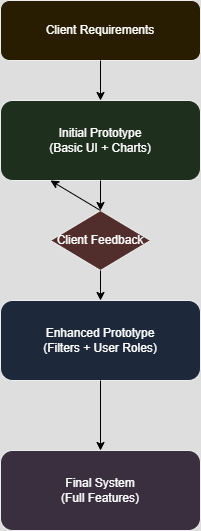
\includegraphics[scale=0.8]{Ch2/Prototype1.png}

\label{fig:Prototype Model}

% Diagram change as per your project demands

\section{Scope of Proposed System}
While in this phase, the scope of em was defined first and then what needs to be done was finalized. Lot of brainstorming ws were very clearly noted down. 
We never came back to revise or change the requirement defined earlier..............

\textbf{Advantages of Proposed System }\\


%\section{Hardware & Software Specifications}


% Write scope of your system.

\section{Technical Specification}
\textbullet \hspace{0.2cm} \textbf{Hardware Specification}\\
Processor	:	Intel(R) Core(TM) i3-7020U CPU @ 2.30GHz 2.30 GHz\\
RAM          	: 	Min. 2GB\\
Hard Disk	: 	Min. 20 GB free\\
% \textbullet \hspace{0.2cm} \textbf{Client}\\
% Processor   	: 	Intel(R) Core(TM) i3-7020U CPU @ 2.30GHz 2.30 GHz\\
% RAM           	: 	Min. 512 MB\\
% Hard Disk	: 	Min. 480 MB free\\
\textbullet \hspace{0.2cm} \textbf{Software Specification}\\
Platform	:  	Windows 11\\
Front End	: 	React.js, Redux (state management). \\
% Middle ware	: 	PHP (Framework : Codeigniter)\\
Back End	: 	Node.js, Express.js. \\	
Database    : MYSQL\\
Web Browser: 	Google Chrome etc. \\


\subsection{Codeignitor Framework}
CodeIgniter is a PHP-driven framework, you churning out dynamic, interactive, professional websites in no time.\\

\textbullet \hspace{0.2cm}	It underpins the Model/View/Controller (MVC) approach to web development—a best practice philosophy all developers should adhere to.\\

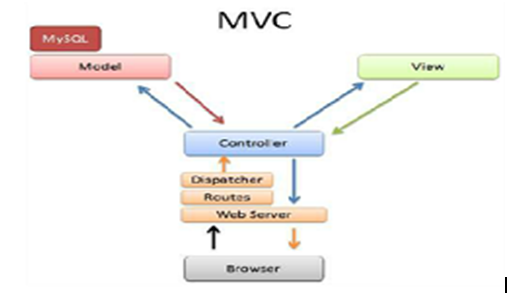
\includegraphics[scale=1.0]{Ch2/mvc.png}


% Diagram change as per your project demands (If required)
\label{fig:MVC Model}

%\textbullet \hspace{0.2cm}It’s built on a linear, easy-to-use folder structure.\\


% This section type your project contents 
\chapter{Feasibility Study}


\section{Introduction}
% the working of the system, \\
% Therefore, a feasibility study of the proposed system needs to be carried out in order to:\\
% \textbullet \hspace{0.2cm} 	Provide a better understanding of the System.\\
% \textbullet \hspace{0.2cm}	Describe the outputs.\\

% There are many factors. These factors are \textbf{Economical Feasibility, Technical Feasibility and Operational Feasibility}.\\

Before building MatricsV, we needed to check if it was actually possible and worthwhile to create. We examined three key areas: cost (can we afford it?), technology (can we actually build it?), and operations (will people use it?). This study helped us understand potential problems before we started coding. We looked at what software we'd need, how much it would cost to run, and whether employees would find it helpful. The results showed that while there would be some challenges in development, the benefits of having clear data visualizations would make the effort worthwhile. Most importantly, we confirmed all the necessary technology was available.



% This section type your project contents 


\section{Economical Feasibility}
% Need not pay any hence the system is economically feasible.\\

The good news is MatricsV doesn't cost much to build! We used free, open-source tools like React.js for the interface and Node.js for the backend, which saved thousands in software fees. Instead of buying expensive servers, we used cloud hosting (AWS) that lets us pay only for what we use. This means if fewer people use the system one month, we pay less. The biggest costs were just the developers' time to build it. Even the charts and graphs use free libraries like Chart.js. Over 3 years, we estimate MatricsV will cost 60% less than buying a ready-made business dashboard system.

% This section type your project contents 
\section{Operational Feasibility}
% company will benefit from the system and hence the system is operationally feasible. \\
We designed MatricsV to be super easy to use, even for non-tech people. The dashboard works like familiar websites - you can drag charts around like moving apps on your phone. Employees only needed 1-2 training sessions because the design is so intuitive. It works with the company's existing computers and doesn't require any special equipment. We tested it with different departments and incorporated their feedback to make it even simpler. The system automatically connects to our current databases, so no manual data entry is needed. Even the CEO, who hates complicated tech, found it easy to understand the sales reports!

\section{Financial and Economical Feasibility}
% % This section type your project contents 
% The economic analysis is the most used........
MatricsV saves the company money in several ways. First, it reduces time spent making reports - what took 5 hours now takes 30 minutes. Second, better data visibility helps managers make smarter decisions, like spotting wasted expenses faster. We calculated that the system paid for itself in just 8 months through these savings. It also reduces errors in manual reporting that used to cost money to fix. While we spent $25,000 developing it, we'll save about $60,000 in the first two years. The finance team approved the project because these numbers show clear financial benefits with very little risk to the company.

\chapter{Proposed System}


\section{Proposed System}
% helps to manage critical processes in Hospital.\\
% \textbf{Patient Registration:} 
%  It provides scheduling/Canceling/Rescheduling of appointments appointment schedule of doctors.\\
% % This section type your project contents 

The proposed system, MatricsV, is designed to provide a modern solution for visualizing complex data through an interactive dashboard. It is user-friendly, scalable, and helps stakeholders easily understand trends and insights. With responsive design, dynamic charts, and real-time filtering, the system meets the needs of both developers and end-users. MatricsV not only enhances data representation but also ensures better performance and usability. The aim of the proposed system is to improve data interpretation and decision-making. It reduces manual effort, ensures efficient data handling, and overcomes the limitations of traditional static dashboards, making data analysis smarter and more accessible.


% \textbf{My Assistant:}
%  My Assistant as a utility performs the role of a personal assistant., It stores information .\\
% % This section type your project contents 



\section{User Privileges}
% The user type determines the privileges that the user has within EHMS.\\

% % This section type your project contents 

\section*{User Privileges}

The proposed system defines clear user privileges to ensure secure and efficient access control within the dashboard environment. Each user role is granted specific rights based on their level of interaction with the system.

\begin{itemize}
    \item \textbf{Admin:}
    \begin{itemize}
        \item Full access to all dashboard features
        \item Manage data sources and chart configurations
        \item Control user access and roles
        \item Perform system-level configurations and updates
    \end{itemize}
    
    \item \textbf{Regular User:}
    \begin{itemize}
        \item View and interact with charts and visualizations
        \item Apply filters and export data
        \item Access assigned datasets and reports
    \end{itemize}
    
    \item \textbf{Guest User (Optional):}
    \begin{itemize}
        \item Limited access to publicly available data views
        \item Read-only access without personalization features
    \end{itemize}
\end{itemize}

These roles ensure data integrity, streamline operations, and maintain security by restricting sensitive functions to authorized users only.


\section{Objective of the System}
% This section type your project contents 

% \begin{itemize}
% \item Latest technology 
% \item Graphical user Interface

The main objective of the system is to develop an interactive and responsive data visualization dashboard that simplifies complex data interpretation. The system aims to provide users with real-time insights through visually intuitive charts and graphs. It is designed to enhance decision-making by presenting data in an organized and accessible manner. Additionally, the system focuses on delivering a seamless user experience across devices, reducing manual effort, and ensuring performance and scalability. Overall, the goal is to bridge the gap between raw data and actionable insights using modern web technologies
\end{itemize}
\chapter{Preliminary  Design}

\section{Tools of data flow strategy}
	% Data flow strategy shows th and their interactions...........\\
	Data flow strategy shows the use of data in the system pictorially. The tools
	use in following this strategy show all the essential features of the system and
	how they fit together. It can be difficult to fully understand a business process
	through a verbal description alone; data flow tools help by illustrating the
	essential components of a system and their interactions.\\
\textbf{Data flow analysis makes use of the following tools:}\\
% Flow Charts\\
% Data Flow Diagrams\\
% Data Dictionary\\
% \textbf{Flowchart}\\
% Flowchart is used to represent the algorithm .......\\
% \textbf{Data Dictionary}\\
% The logical characteristics of current systems data stores, including name, description, aliases, contents, ..........\\
% \textbf{Data Structure Diagrams}\\
% A pictorial description of the relation between entities (people, places, events and things) in system and the set of information about the entity, .........\\
% \textbf{Structured Chart}\\
% A design tool that pictorially shows the relation between processing modules in computer software, describes .............

\begin{itemize}
    \item \textbf{Use Case Diagram}:\\
    Illustrates the interactions between users (actors) and the system, showcasing the functional requirements and major processes.

    \item \textbf{Data Flow Diagrams (DFD)}:\\
    Represent the flow of data within the system. DFDs help visualize how information moves between processes, data stores, and external entities.

    \item \textbf{Entity Relationship Diagram (ER-Diagram)}:\\
    Displays the logical structure of the database, showing entities, attributes, and the relationships among them. It is crucial for designing a consistent and efficient database schema.
\end{itemize}
%-----------------------------------------------------------------

\section{Use Case Diagram}
%If you add information about use case diagram\\
\subsubsection{Usecase Diagram For Admin}
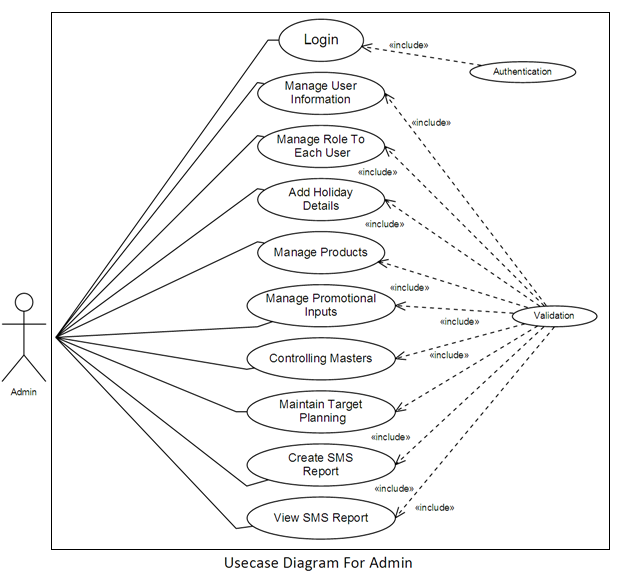
\includegraphics[scale=0.7]{Diag/usecaseadmin.png}

\label{fig:Use case diagram For Admin}
\subsubsection{Usecase Diagram For Other Users.}
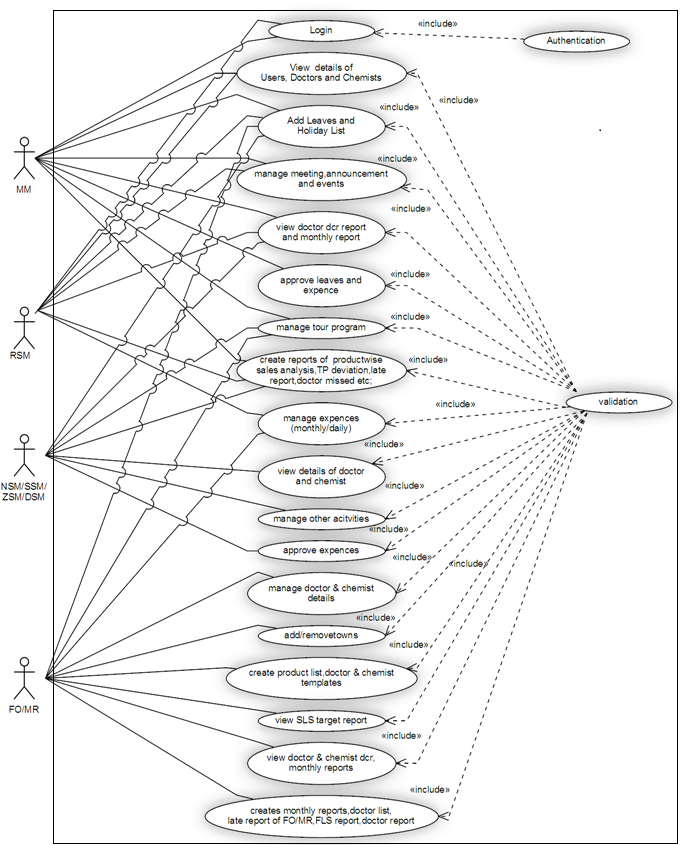
\includegraphics[scale=0.8]{Diag/usecaseall.png}

\label{fig:Use case diagram For Other User}



%-----------------------------------------------------------------
%\section{Activity Diagram}
%%If you add information about Activity Diagram\\
%
%\includegraphics[scale=.8]{Diag/activitylogin.png}
%\label{fig:Activity Diagram}



%-----------------------------------------------------------------

\section{Entity Relationship Diagram}

\subsubsection{ERD For Chemist.}
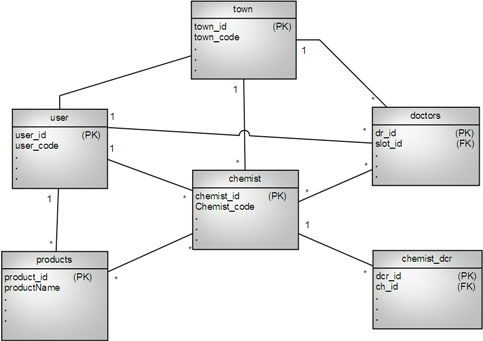
\includegraphics[scale=0.7]{Diag/ERDchemist.png}
\label{abc}

\subsubsection{ERD For doctor.}
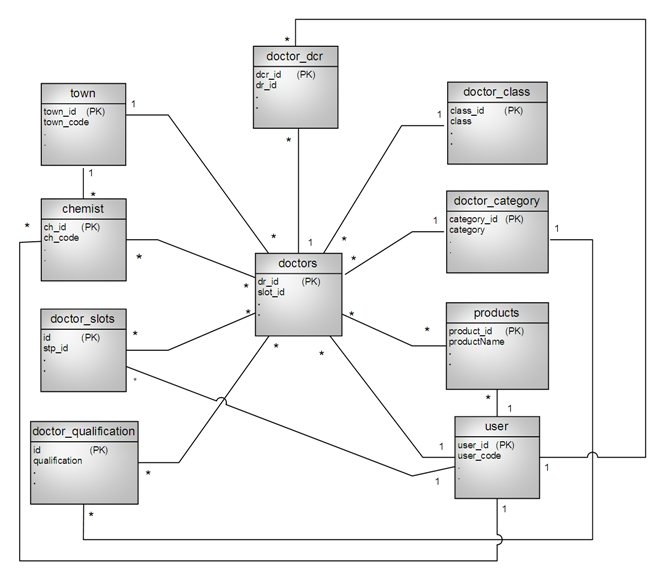
\includegraphics[scale=0.7]{Diag/ERDdoctor.png}
\label{abc}


%\subsubsection{ERD For users.}
%\includegraphics[scale=0.7]{Diag/ERDuser.png}
%\label{abc}
%
%\subsubsection{ERD For Products.}
%\includegraphics[scale=0.7]{Diag/ERDprod.png}
%\label{abc}
%-----------------------------------------------------------------

\section{Data Flow Diagram}
%If you add information about Data flow diagram\\

%\begin{figure} [h]
%\begin{center} 
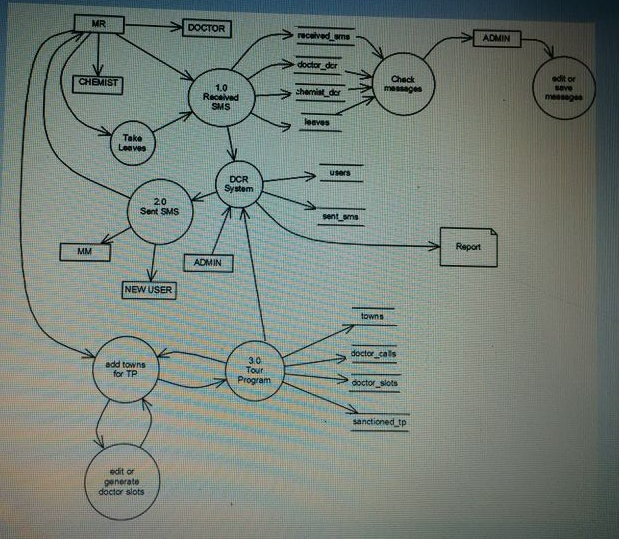
\includegraphics[scale=.9]{Diag/d1.png}
\label{fig:Contex Level}
%\end{center}
%\end{figure}



%\begin{figure} [h]
%\begin{center} 
%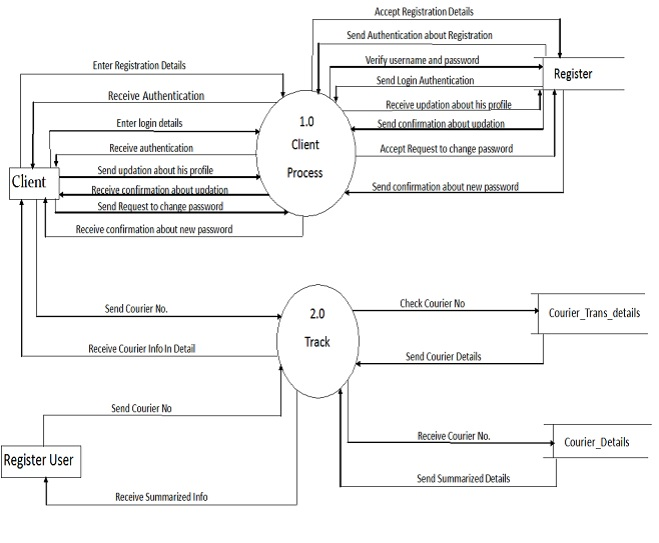
\includegraphics[scale=.9]{Ch5/dfd2.jpg}
%Fig. Data Flow Diagram
%\label{fig:DFD2}


\
% Students should divide chapter 3,4,5 according to major blocks of their project
\chapter{Detailed Design}

Simply functionality and availability, is selected based on the relative important of these criteria.............. 

\section{Data Dictionary}
                                    Data dictionary is only collection of data element definition. Entries in a data dictionary include the name of the data item and attributes. ...........

\section{Input and output Design}

		Considering all o the interaction of user with the system be in most effective and simplified way.                All the input forms are designed in she user will be able to use them in very eff possibilities needed by the user................
		
		
		% This section type your project contents 
		
		
		
\subsection{Admin}
\pagebreak
\textbf{login}
\begin{center}
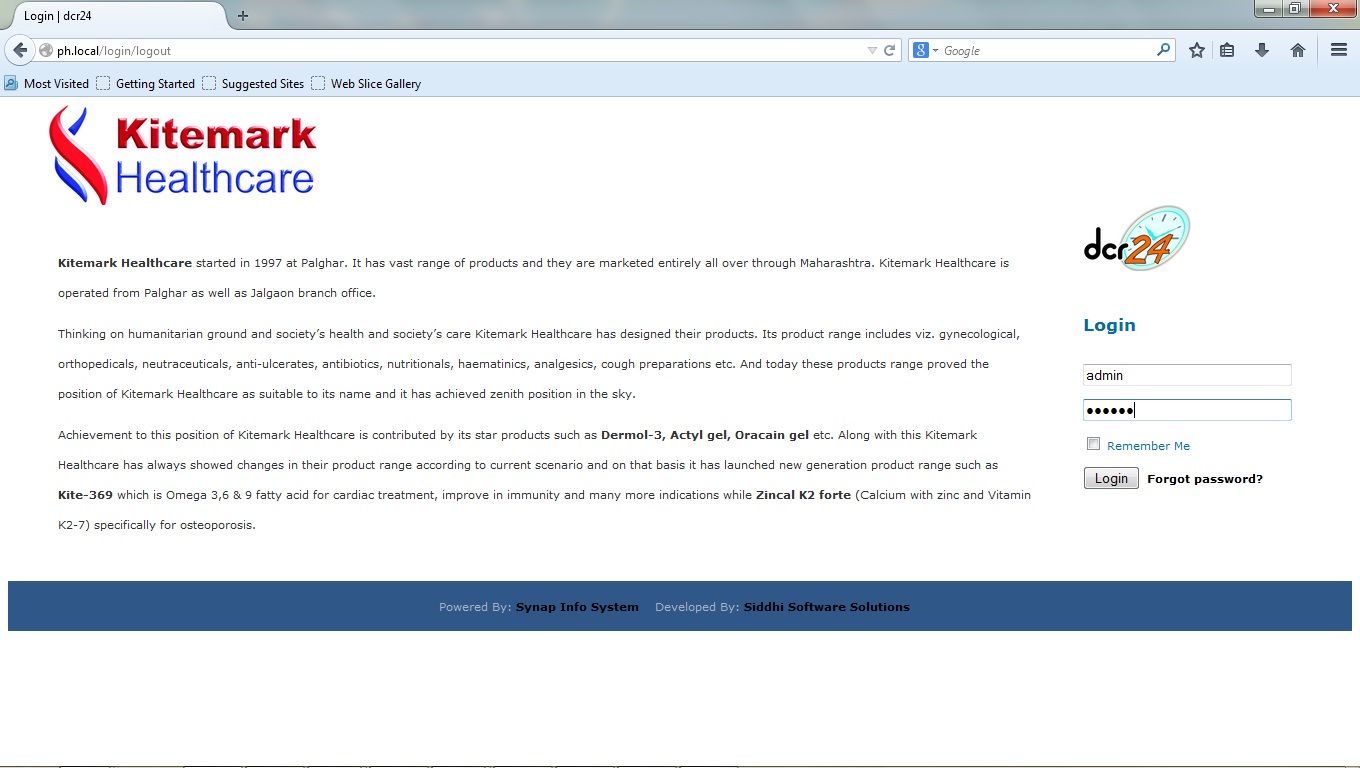
\includegraphics[height=9cm,width=14cm]{Admin/login.jpg}
\end{center}


% This section type your project contents 

\textbf{Admin Dashboard}
\begin{center}
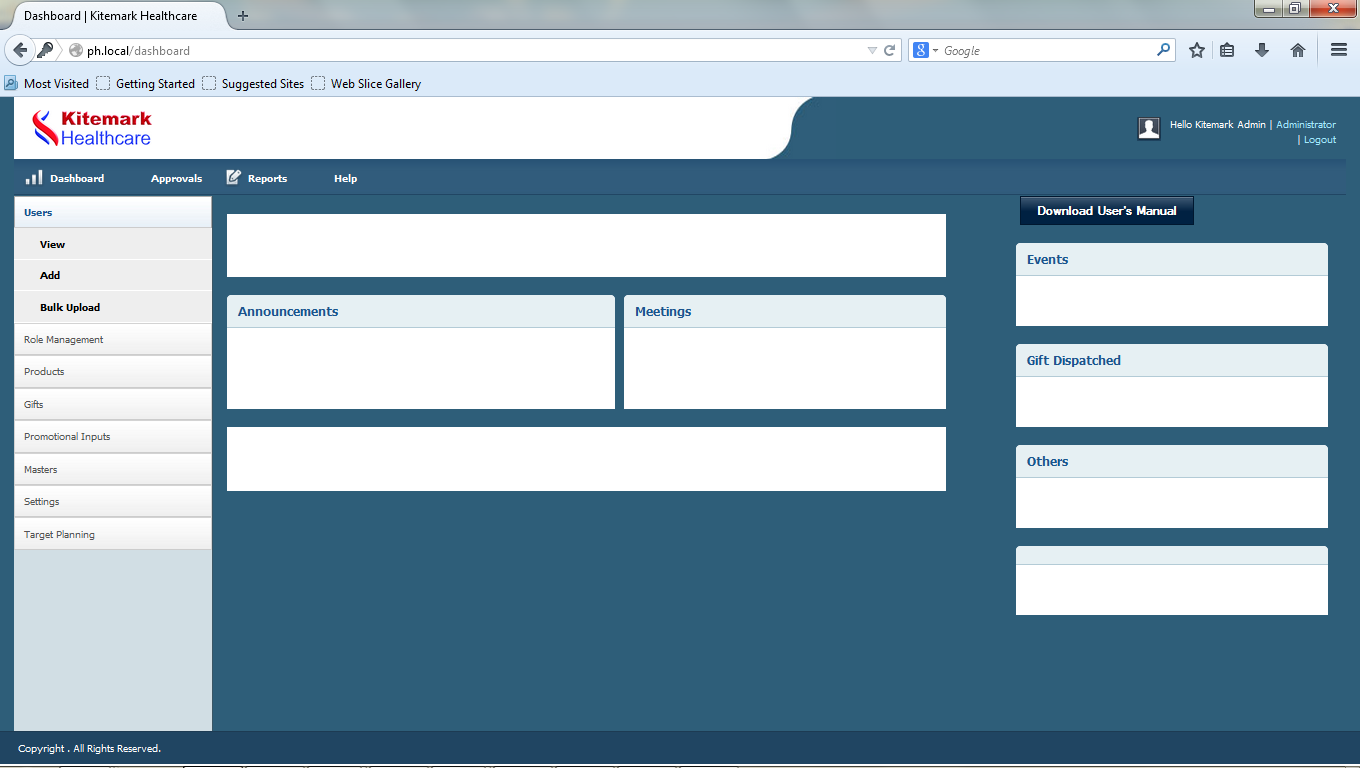
\includegraphics[height=9cm,width=14cm]{Admin/dashboard.png}
\end{center}
\pagebreak

\textbf{View Users}
\begin{center}
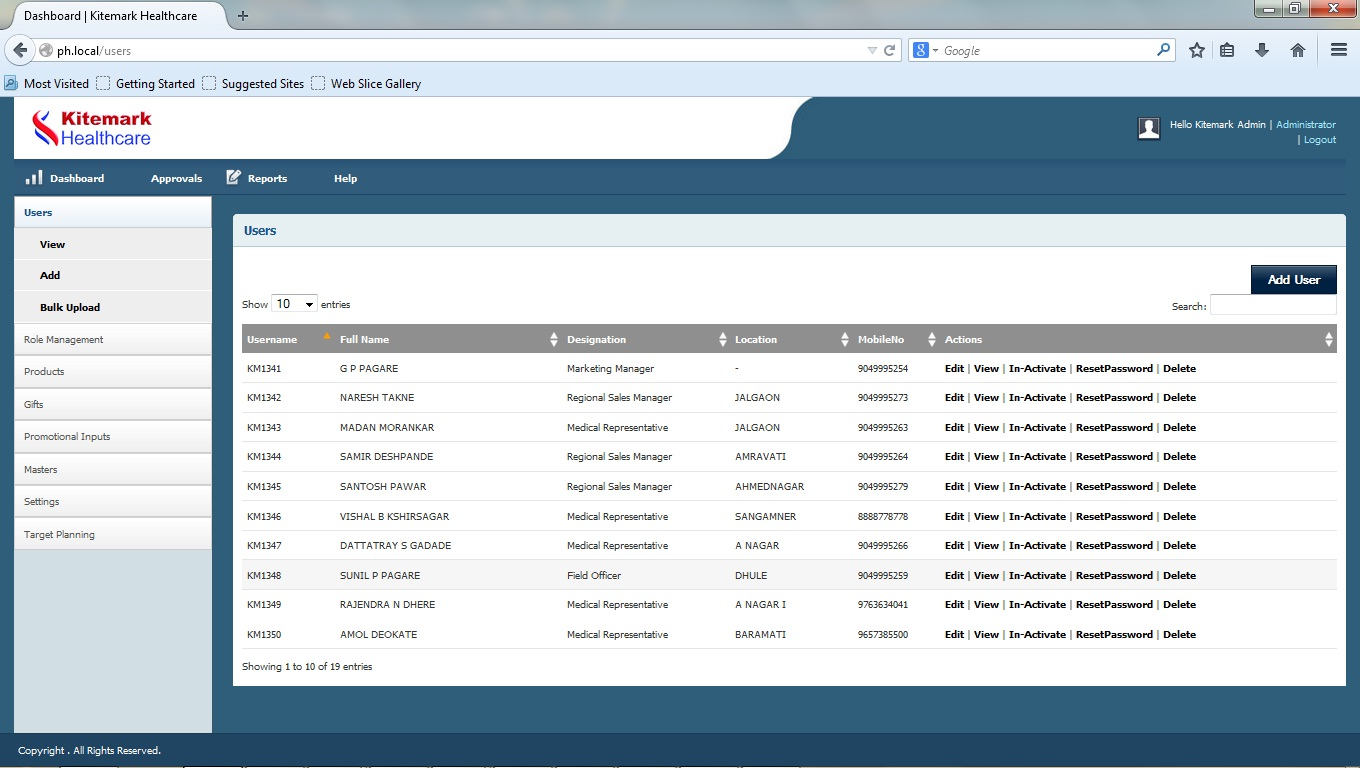
\includegraphics[height=9cm,width=14cm]{Admin/viewusers.jpg}
\end{center}



% This section type your project contents 
\textbf{Add User}
\begin{center}
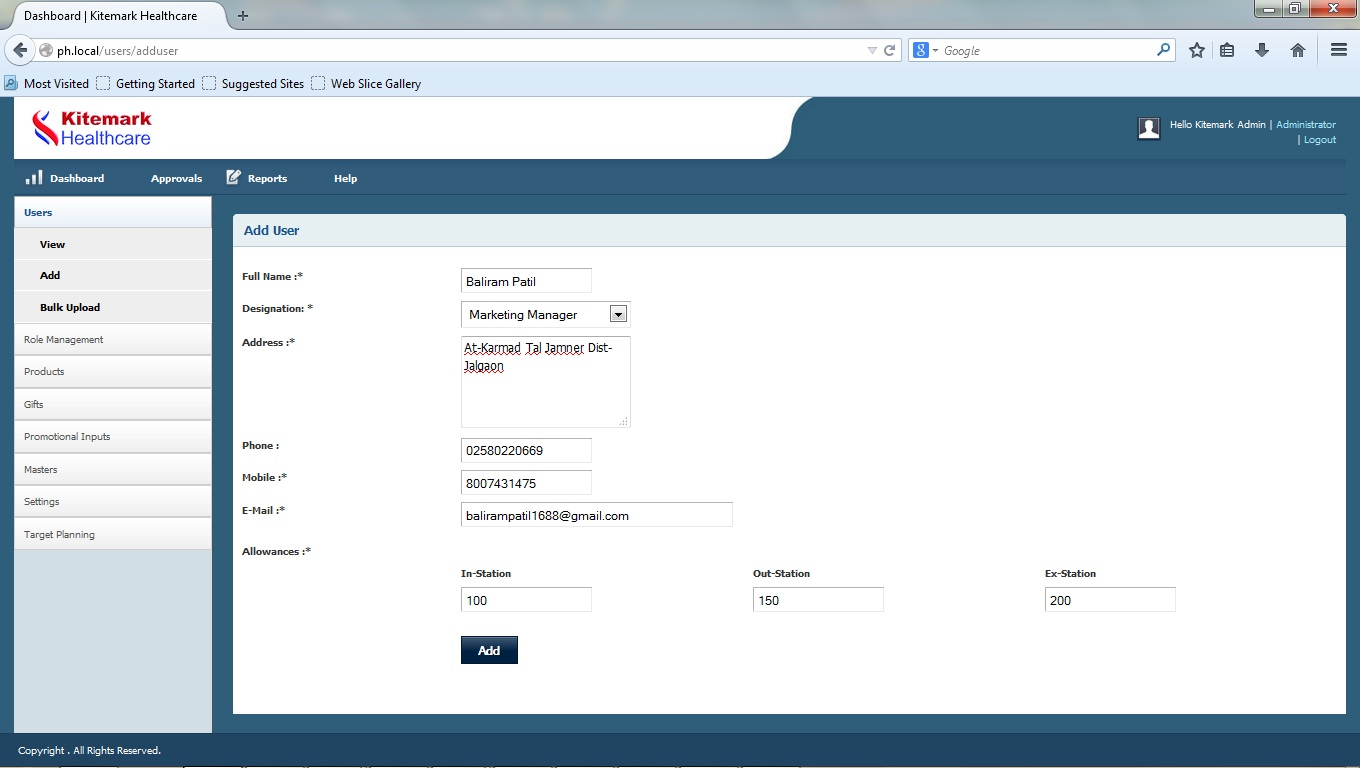
\includegraphics[height=9cm,width=14cm]{Admin/addusers.jpg}
\end{center}
\pagebreak

		
		% This section type your project contents 
		
		
		
		
		
		
		
		
		
		
		
		
		
		
		
		
		
		
		
		
		
		
		
		
		
		
		
 		

\section{Database structure}
\textbf{announcement:}  This table stores announcement added by Admin and useful to display announcement to other users.\nolinebreak
\begin{table}[hp]
\centering

\begin{tabular}{|c|c|c|c|}
\hline
\textbf{Field Name}  & \textbf{Data Type}  & \textbf{size} &\textbf{Constraints}  \\
\hline
announceid & int & 20 & Primary Key,auto\_increment \\
\hline
title &	varchar &	200 & NOT NULL.\\
\hline
description & varchar &	255 & NOT NULL.\\
\hline
addedBy	& int & 11 &	NOT NULL\\
\hline
addedon &	datetime &	- &	NOT NULL.\\
\hline
updatedon &	datetime &	- &	NOT NULL.\\
\hline
expiry\_date & date & 20 & NOT NULL.\\
\hline
status	& varchar &	- & NOT NULL. \\
\hline

\end{tabular}
\caption{ announcement}
\end{table}
\\
\textbf{area:} This table stores area details with region of that area.\nolinebreak
\begin{table}[hp]
\centering
\begin{tabular}{|c|c|c|c|}
\hline
\textbf{Field Name}  & \textbf{Data Type}  & \textbf{size} &\textbf{Constraints}  \\
\hline
area\_id & bigint &	20 & Primary Key,auto\_increment\\
\hline
area &	varchar &	25 & NOT NULL \\
\hline
region\_id &	bigint & 20 & NOT NULL \\
\hline
isActive &	int & 	11  & NOTNULL \\
\hline
addedon & datetime & - & NOT NULL\\
\hline
updatedon &	datetime & - & NOT NULL\\
\hline
\end{tabular}
\caption{area}
\end{table}

\pagebreak
\textbf{chemist:}  This table stores all chemist details added by Medical Representative or Field Officer.\nolinebreak

\begin{table}[hp]
\centering
\begin{tabular}{|c|c|c|c|}
\hline
\textbf{Field Name}  & \textbf{Data Type}  & \textbf{size} &\textbf{Constraints}  \\
\hline
chemist\_id & bigint &	20 & Primary Key,auto\_increment\\
\hline
chemist\_code &	bigint & 20 & NOT NULL\\
\hline
store\_name	& varchar &	100 & NOT NULL\\
\hline
store\_address &	Text &	- & NOT NULL\\
\hline
town\_id & bigint & 	20 & NOT NULL\\
\hline
contact\_person & varchar & 100 & NOT NULL\\
\hline
mobile & varchar & 12 & NOT NULL\\
\hline
email &	varchar & 100 & NOT NULL\\
\hline
dob & date & - & NOT NULL\\
\hline
date\_of\_marrige & date & - & NOT NULL\\
\hline
is\_hospital\_attached & tinyint & 	2 & NOT NULL\\
\hline
hospital\_name &	varchar &	100 & NOT NULL\\
\hline
dr\_of\_hospital &	varchar &	100 & NOT NULL\\
\hline
near\_by\_dr & varchar &	100 & NOT NULL\\
\hline
available\_products &	varchar &	150 & NOT NULL\\
\hline
monthly\_purchase &	bigint & 20 & NOT NULL\\
\hline
status & varchar & 20 & NOT NULL\\
\hline
approved\_by & varchar &	25 & NOT NULL\\
\hline
reject\_reason & varchar & 200 & NOT NULL\\
\hline
added\_by &	bigint & 20 & NOT NULL\\
\hline
added\_on &	datetime &	- & NOT NULL\\
\hline
updated\_by & bigint &	20 & NOT NULL\\
\hline
updated\_on &	datetime &	- & NOT NULL\\
\hline
isActive &	tinyint &	2 & NOT NULL\\
\hline
\end{tabular}
\caption{chemist}
\end{table}


\textbf{target\_product\_sale} This table stores the target of product sales .\nolinebreak
\begin{table}[hp]
\centering
\begin{tabular}{|c|c|c|c|}
\hline
\textbf{Field Name}  & \textbf{Data Type}  & \textbf{size} &\textbf{Constraints}  \\
\hline
id &	bigint &	20 & Primary Key,auto\_increment \\\hline
year &	 int &	11 & NOT NULL \\\hline
hq\_id	 & int &	11 & NOT NULL \\\hline
prod\_id &	bigint &	20 & NOT NULL \\\hline
sale &	double &	- & NOT NULL \\\hline
 added\_by &	bigint &	20 & NOT NULL \\\hline
added\_on &	datetime &	- & NOT NULL \\\hline
updated\_by &	bigint &	20 & NOT NULL \\\hline
updated\_on &	datetime &	- & NOT NULL \\\hline

 
\end{tabular}
\caption{target\_product\_sale}
\end{table}

\textbf{target\_prod\_calculations} This table stores the product wise  target calculation.\nolinebreak
\begin{table}[hp]
\centering
\begin{tabular}{|c|c|c|c|}
\hline
\textbf{Field Name}  & \textbf{Data Type}  & \textbf{size} &\textbf{Constraints}  \\
\hline
id &	bigint &	20 & Primary Key,auto\_increment \\\hline
year &	int &	11 & NOT NULL \\\hline
prod\_id &	bigint &	20 & NOT NULL \\\hline
packing &	varchar &	100 & NOT NULL \\\hline
calc\_value &	double &	- & NOT NULL \\\hline
expected\_growth &	double &	- & NOT NULL \\\hline
min1 &	double &	- & NOT NULL \\\hline
 min2 &	double &	- & NOT NULL \\\hline
  min3 &	double &	- & NOT NULL \\\hline
  added\_by &	bigint &	20 & NOT NULL \\\hline
added\_on &	datetime &	- & NOT NULL \\\hline
updated\_by &	bigint &	20 & NOT NULL \\\hline
updated\_on	 & datetime &	- & NOT NULL \\\hline

 
\end{tabular}
\caption{target\_prod\_calculations}
\end{table}

\textbf{target\_sls} This table stores the  target of sls.\nolinebreak
\begin{table}[hp]
\centering
\begin{tabular}{|c|c|c|c|}
\hline
\textbf{Field Name}  & \textbf{Data Type}  & \textbf{size} &\textbf{Constraints}  \\
\hline
id &	int	 & 11 & Primary Key,auto\_increment \\\hline
month &	text &	 & NOT NULL \\\hline
hq\_id &	int &	11 & NOT NULL \\\hline
product\_id &	int &	11 & NOT NULL \\\hline
sls &	bigint &	20 & NOT NULL \\\hline
closing\_stock &	bigint &	20 & NOT NULL \\\hline
added\_by &	bigint &	20 & NOT NULL \\\hline
added\_on &	datetime &	- & NOT NULL \\\hline
updated\_by &	bigint &	20 & NOT NULL \\\hline
updated\_on &	datetime &	- & NOT NULL \\\hline
monthno &	int &	11 & NOT NULL \\\hline
year &	int &	11 & NOT NULL \\\hline

 
\end{tabular}
\caption{target\_sls}
\end{table}

\pagebreak

\textbf{target\_yearly} This table stores the  yearly target.\nolinebreak
\begin{table}[hp]
\centering
\begin{tabular}{|c|c|c|c|}
\hline
\textbf{Field Name}  & \textbf{Data Type}  & \textbf{size} &\textbf{Constraints}  \\
\hline
id &	int &	11 & Primary Key,auto\_increment \\\hline
year &	  text &	 & NOT NULL \\\hline
hq\_id &	int &	11 & NOT NULL \\\hline
product\_id &	int &	11 & NOT NULL \\\hline
annual\_target &	bigint &	20 & NOT NULL \\\hline
target\_value	& bigint &	20 & NOT NULL \\\hline
intro\_month &	text &	- & NOT NULL \\\hline
added\_by &	bigint &	20 & NOT NULL \\\hline
added\_on &	datetime &	- & NOT NULL \\\hline
updated\_by &	bigint &	20 & NOT NULL \\\hline
updated\_on &	datetime &	- & NOT NULL \\\hline
 
\end{tabular}
\caption{target\_yearly}
\end{table}

\textbf{town} This table stores the  town details.\nolinebreak
\begin{table}[hp]
\centering
\begin{tabular}{|c|c|c|c|}
\hline
\textbf{Field Name}  & \textbf{Data Type}  & \textbf{size} &\textbf{Constraints}  \\
\hline
 town\_id	& bigint &	20 & Primary Key,auto\_increment \\\hline
 town\_code &	bigint	 & 20 & NOT NULL \\\hline
town &	 varchar &	25 & NOT NULL \\\hline
hq\_id &	bigint &	20 & NOT NULL \\\hline
isActive &	tinyint &	11 & NOT NULL \\\hline
status &	varchar &	20 & NOT NULL \\\hline
approved\_by &	varchar &	25 & NOT NULL \\\hline
reject\_reason &	varchar &	200 & NOT NULL \\\hline
added\_by &	bigint &	20 & NOT NULL \\\hline
added\_on &	datetime &	- & NOT NULL \\\hline
updated\_by &	bigint &	20 & NOT NULL \\\hline
updated\_on &	datetime &	- & NOT NULL \\\hline
 
\end{tabular}
\caption{town}
\end{table}

\textbf{users} This table stores the users details.\nolinebreak
\begin{table}[hp]
\centering
\begin{tabular}{|c|c|c|c|}
\hline
\textbf{Field Name}  & \textbf{Data Type}  & \textbf{size} &\textbf{Constraints}  \\
\hline
 id &	int &	11 & Primary Key,auto\_increment \\\hline
company\_code &	varchar &	3 & NOT NULL \\\hline
username &	varchar &	25 & NOT NULL \\\hline
password &	varchar &	25 & NOT NULL \\\hline
fullname &	varchar &	50 & NOT NULL \\\hline
role\_id &	int &	11 & NOT NULL \\\hline
reports\_to &	int &	11 & NOT NULL \\\hline
address &	varchar &	50 & NOT NULL \\\hline
phone &	varchar	 & 25 & NOT NULL \\\hline
mobile &	varchar &	10 & NOT NULL \\\hline
email &	varchar &	50 & NOT NULL \\\hline
nation\_id &	int &	20 & NOT NULL \\\hline
zone\_id &	bigint &	20 & NOT NULL \\\hline
state\_id &	bigint &	20 & NOT NULL \\\hline
division\_id &	bigint &	20 & NOT NULL \\\hline
region\_id &	bigint &	20 & NOT NULL \\\hline
area\_id &	bigint &	20 & NOT NULL \\\hline
headQuarter\_id &	bigint &	20 & NOT NULL \\\hline
based\_on &	varchar &	50 & NOT NULL \\\hline
addedBy &	bigint &	20 & NOT NULL \\\hline
addedOn &	datetime &	- & NOT NULL \\\hline
updatedOn &	datetime &	- & NOT NULL \\\hline
 isActive &	tinyint &	1 & NOT NULL \\\hline
instation &	int &	11 & NOT NULL \\\hline
outstation &	int &	11 & NOT NULL \\\hline
exstation &	int &	11 & NOT NULL \\\hline

\end{tabular}
\caption{users}
\end{table}

\textbf{users\_leave} This table stores the userwise leave details.\nolinebreak
\begin{table}[hp]
\centering
\begin{tabular}{|c|c|c|c|}
\hline
\textbf{Field Name}  & \textbf{Data Type}  & \textbf{size} &\textbf{Constraints}  \\
\hline
user\_id &	int &	11 &  Primary Key,auto\_increment \\\hline
holiday\_id &	int &	11 & NOT NULL \\\hline
date & date &	- & NOT NULL \\\hline

\end{tabular}
\caption{users\_leaves}
\end{table}

\textbf{users\_profile} This table stores the user profiles details.\nolinebreak
\begin{table}[hp]
\centering
\begin{tabular}{|c|c|c|c|}
\hline
\textbf{Field Name}  & \textbf{Data Type}  & \textbf{size} &\textbf{Constraints}  \\
\hline
profile\_id &	int &	11 &  Primary Key,auto\_increment \\\hline
profile\_name &	varchar &	50 & NOT NULL \\\hline
discription  & varchar &	200 & NOT NULL \\\hline

\end{tabular}
\caption{users\_profile}
\end{table}

\pagebreak

\textbf{user\_roles} This table stores the user roles details.\nolinebreak
\begin{table}[hp]
\centering
\begin{tabular}{|c|c|c|c|}
\hline
\textbf{Field Name}  & \textbf{Data Type}  & \textbf{size} &\textbf{Constraints}  \\
\hline
role\_id &	int &	11 & Primary Key,auto\_increment \\\hline
profile\_id &	varchar &	3 & NOT NULL \\\hline
 parent\_id &	varchar &	25 & NOT NULL \\\hline
designation &	varchar &	25 & NOT NULL \\\hline
permission &	varchar &	50 & NOT NULL \\\hline
isActive &	int &	11 & NOT NULL \\\hline
added\_by	 & bigint	& 20 & NOT NULL \\\hline
added\_on	 & datetime &	- & NOT NULL \\\hline
updated\_by &	bigint &	20 & NOT NULL \\\hline
updated\_on &	datetime &	- & NOT NULL \\\hline
  

\end{tabular}
\caption{users\_roles}
\end{table}

\textbf{zones} This table stores the zones details.\nolinebreak
\begin{table}[hp]
\centering
\begin{tabular}{|c|c|c|c|}
\hline
\textbf{Field Name}  & \textbf{Data Type}  & \textbf{size} &\textbf{Constraints}  \\
\hline
zone\_id &	bigint &	20 & Primary Key,auto\_increment \\\hline
title &	varchar &	25 & NOT NULL \\\hline
 nation\_id &	int &	11 & NOT NULL \\\hline
isActive &	 int &	11 & NOT NULL \\\hline
addedOn &	datetime &	- & NOT NULL \\\hline

\end{tabular}
\caption{zones}
\end{table}


\chapter{Testing}


\section{Introduction}\\
Testing is a process of executing error. It is an important and critical stage in software development. It plays an important role in determining the quality and reliability of the application. With this process, several test cases are devised. A test case means a set of data that the system will process as the normal input. Testing also adds value to the product by conforming the user requirements. Testing verifies that this software deliverable conforms precisely to the functional and design specification that have been compiled during analysis and design phases. A good test case is one that has a high portability of finding an undiscovered error. Testing involves a series of operation of a system or application under controlled conditions and subsequently evaluating results. The controller conditions should include both normal and abnormal conditions. It is planned and monitors for each testing level.

% Testing is a process of executing error. A good test is the ......\\ 
%  The increasing  a software failure are motivating forces for well planned, through testing...........\\

% This section type your project contents 

\section{White Box Testing}
This testing reveals the internal working of the code i.e. each of the programming elements is exercised properly. The white box testing for the proposed system focus on the program control structure and it is also called clear box testing. Test cases for the proposed system are designed to ensure that all statements in the program have executed at least once during testing and that all logical conditions have been exercised. White box testing is small implying that this test is typically applied to small program components.




% This section type your project contents 

\section{Black Box Testing}
Black Box Testing was conducted to ensure the MatricsV dashboard met functional requirements without examining internal code. The testing focused on input-output validation, such as verifying that charts updated correctly with filters, views rendered properly, and the interface was responsive across devices. Key scenarios included testing chart behavior, data filtering, error handling, and navigation. For example, applying a date filter correctly updated all relevant charts, while mobile view tests ensured proper layout adjustments. Issues like stale chart props and overflow bugs were identified and resolved. This testing approach ensured a smooth, user-focused experience and reliable functionality across different environments.


% This section type your project contents 


\section{Validation Testing}
Validation Testing was performed to ensure the MatricsV dashboard met all specified requirements and user expectations. Each feature, including data visualization, filtering, responsiveness, and navigation, was verified against the original project scope. Charts were tested with dynamic datasets to confirm accurate rendering, and filters were validated for correct interaction. Responsive design was checked across devices to ensure consistent usability. The final product successfully passed all validation checks, confirming it aligned with the intended functionality and design. This process guaranteed that the application not only worked correctly but also delivered a user-centric and purpose-driven experience.

% This section type your project contents 

\section{GUI Testing}
GUI Testing was conducted to ensure the visual elements of the MatricsV dashboard functioned correctly and provided a seamless user experience. All user interface components—charts, filters, dropdowns, date pickers, and navigation tabs—were tested for proper alignment, styling, responsiveness, and interactivity. Tailwind CSS utilities were verified across screen sizes to confirm consistent design. Focus was placed on color schemes, font consistency, hover effects, and button functionality. Interactive elements responded accurately to user actions without layout shifts or overlap issues. The testing confirmed that the dashboard maintained both aesthetic quality and usability across different browsers and devices.



% This section type your project contents 
\chapter{Concluding Remarks}


\section{Strengths of System}
The MatricsV dashboard is designed to be easy to use, featuring a clean and user-friendly graphical interface. Users can quickly navigate through the system and easily locate menu items, reducing time and effort. The intuitive design enhances user satisfaction by allowing them to generate a variety of reports tailored to their needs. Fast data access and responsive charts make information retrieval efficient and effective. Overall, the system supports seamless interaction, faster decision-making, and an improved user experience, making it a valuable tool for visual data analysis.
% \begin{enumerate}
% \item 1.	System is easy to use....
% \item 2.	System has a user friendly GUI...


\end{enumerate}
% This section type your project contents 

\section{Limitations of system}

\begin{itemize}
\item 1.	The only limitation of the system is that the system is not fully automated....
\item 2.	The limited scope of current System doesn’t fully encompass the current system.....


% This section type your project contents 
\end{itemize}

\section{Scope for future development} 

In future development, we can add a printer integration feature for easy record printing. More advanced software for Octaculus Learning can be introduced, offering additional facilities. Hosting the platform on online servers will make it accessible worldwide. A backup mechanism can be implemented to regularly secure the codebase and database on different servers. We can also expand the project to maintain assignment and student records efficiently. Considering the growing versatility of learners, a dedicated module to manage Octaculus Learning activities can be developed. These enhancements will increase the applicability, usability, and overall value of the platform.

% This section type your project contents 

\section{Conclusion}
The Data Visualization project was a rewarding experience that provided a solid foundation in both frontend development and data representation techniques. The project's real-world relevance and practical application strengthened my confidence in designing and implementing modern web applications. It was an excellent opportunity to transition from theoretical learning to practical execution. I believe this project will serve as a stepping stone toward more advanced analytics applications, and I look forward to building even more sophisticated systems that merge data and design effectively.

% \begin{itemize}
% \item	Pharma Sales Force Automation (PsfA) is the product whir planning and provide more time for work tal organizations....
% \item	The main motive of learning and acquiring the skills has also been achieved. \\
% o	Way of analyzing the system.\\

% % This section type your project contents 
% o	Importance and skill of proper database design.\\
% o	Proper use of state management tools.\\

% % This section type your project contents 

% \item	Company too is satisfied with the quality of work.

% \end{itemize}
%\addcontentsline{toc}{chapter}{References}


%\chapter*{Appendix}

% Students are write appendix then write here., Otherwise Comment this chapter in chapter list (Select main.tex file and comment in front of appendix chapter)


\addcontentsline{toc}{chapter}{Appendix}
%\textbf{\centerline{Appendix}}	\\
\chapter*{\centerline{Appendix}}
\newpage
   % Not required then comment only 
\addcontentsline{toc}{chapter}{References}
\renewcommand\bibname{References}
\begin{thebibliography}{99}



% This section type your project contents 


\bibitem{Books} Books Referred,\\
Following books proved to be very helpful during the development of the system.\\
•	CodeIgnitor for Rapid PHP Application Developement\\
David Upton\\
•	Software Engineering: A Practitioner’s Approach, Seventh Edition
Roger S. Pressman\\
\bibitem{Web} WebSites Visited :-\\
Following websites proved to be very helpful during the development of the system.\\
•	www.msdn.microsoft.com\\
•	www.w3schools.com\\
•	www.codeproject.com\\


% This section type your project contents 

\bibitem{diagrams} Software Used for Diagrams\\
•	Pacestar UML Diagrammer 6

% This section type your project contents 
\bibitem{SoftEng} Software Engineering a Practitioner’s Approach. (McGraw Hill Publication) 		Roger S. Pressman.
% This section type your project contents 
\end{thebibliography}
% ---------------------------------------------------------------------------------
% if any table wants to add in any chapter use following
%
%			\begin{table}[!ht]
%			\caption{Initial Testing Without Samples }   % name of table to be displayed above 						%											 				   table and in List of tables
%			\begin{tabular}{ c  c  c  c }				% table having 4 column
%							1 & 10 & 20 & 30 \\ 		% entries of column can separated by using &
%							2 & 40 & 50 & 60 \\ 		
%			\end{tabular}
%			\label{result1}		% for calling table no. in text
% 			\end{table} 
%
% ---------------------------------------------------------------------------------
\end{spacing}
\end{document}
